\chapter{Estructura del Espacio de Trabajo}

\section{Disposición General}

El núcleo de la aplicación \textit{MDAA} reside en el espacio de trabajo que se habilita al abrir un proyecto. Esta vista está diseñada para maximizar la eficiencia y organizar lógicamente todas las herramientas necesarias para la definición de sintetizadores musicales.



\begin{figure}[!ht]
    \centering
    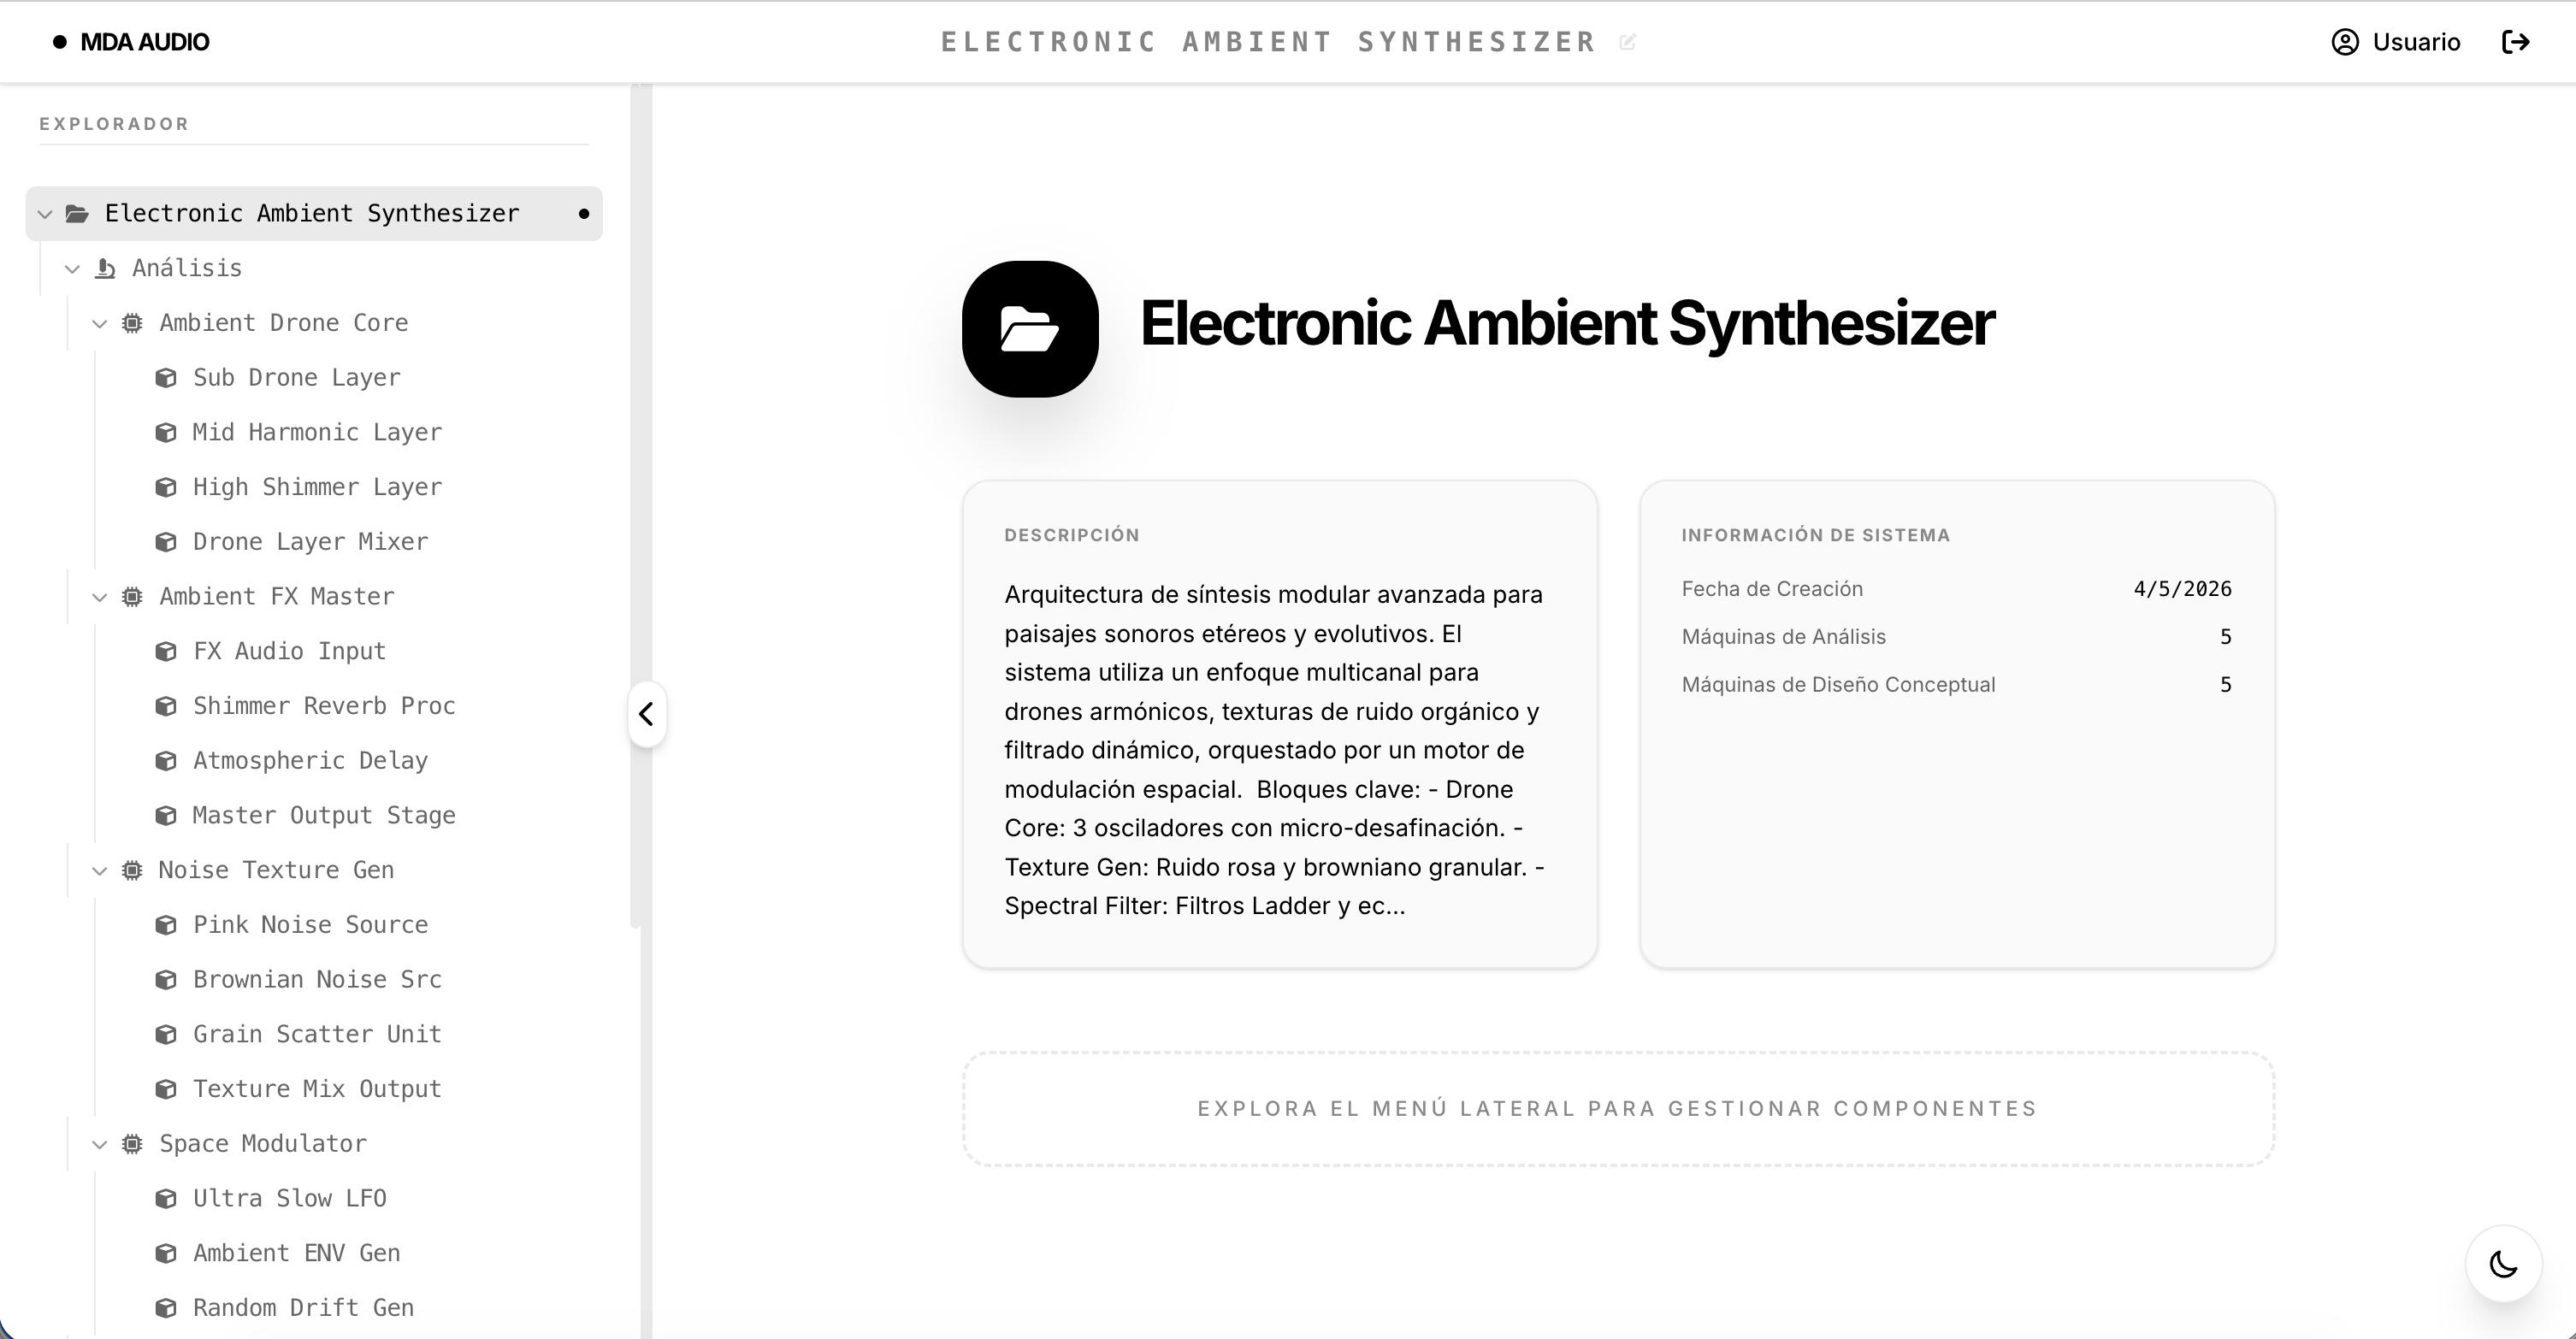
\includegraphics[width=\textwidth]{imagenes/04_estructura/01_pantallaPrincipalProyectoConSus3Partes.png}
    \caption{Pantalla principal del proyecto dividida en tres áreas fundamentales.}
\end{figure}

La interfaz del espacio de trabajo se divide estructuralmente en tres partes principales:
\begin{itemize}
    \item \textbf{Barra Principal Superior:} Contiene controles globales de navegación, gestión de la vista y acciones críticas del proyecto.
    \item \textbf{Explorador del Proyecto (Panel Izquierdo):} Muestra la estructura jerárquica de los elementos del proyecto, facilitando la navegación entre modelos de análisis y diseño.
    \item \textbf{Área de Trabajo Central:} Es el lienzo principal donde se abren los editores visuales y textuales para interactuar con los elementos del dominio.
\end{itemize}

\subsection{El Explorador del Proyecto}

El explorador es el panel lateral que organiza el contenido. Funciona como un árbol de directorios que clasifica los modelos según la metodología \textit{MDAA}.

\begin{figure}[!ht]
    \centering
    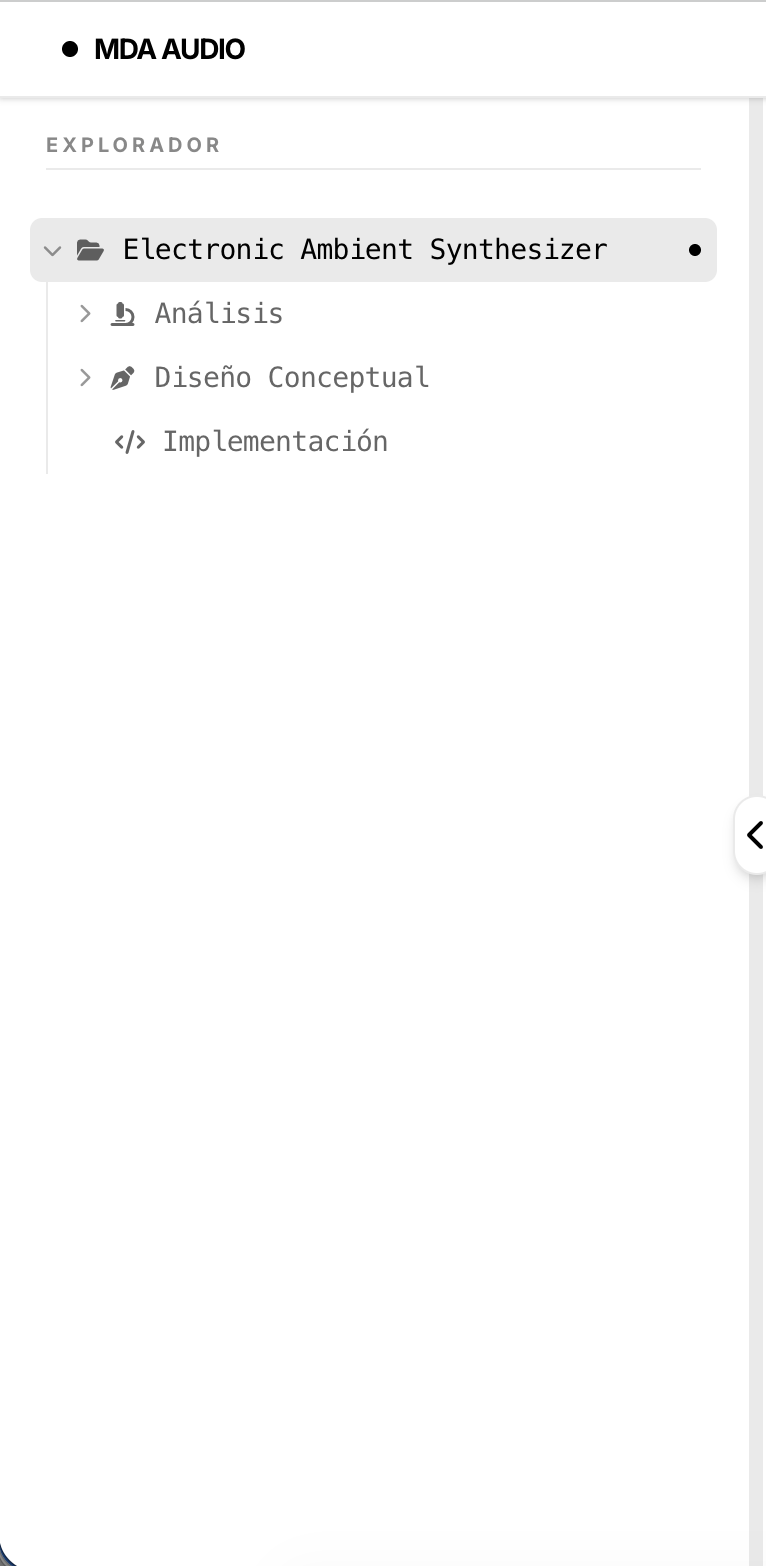
\includegraphics[width=0.4\textwidth]{imagenes/04_estructura/03_exploradorDelProyecto.png}
    \caption{Detalle del explorador jerárquico del proyecto.}
\end{figure}

En el explorador se distinguen claramente dos ramas principales:
\begin{itemize}
    \item \textbf{Análisis Conceptual (CIM):} Donde se definen los modelos independientes de la computación, capturando los requerimientos del dominio musical.
    \item \textbf{Diseño Conceptual (PIM):} Donde se establece la arquitectura independiente de plataforma, basándose en el análisis previo.
\end{itemize}
Al pulsar sobre cualquier elemento del árbol, este se abre como una pestaña en el área de trabajo central.

\begin{figure}[!ht]
    \centering
    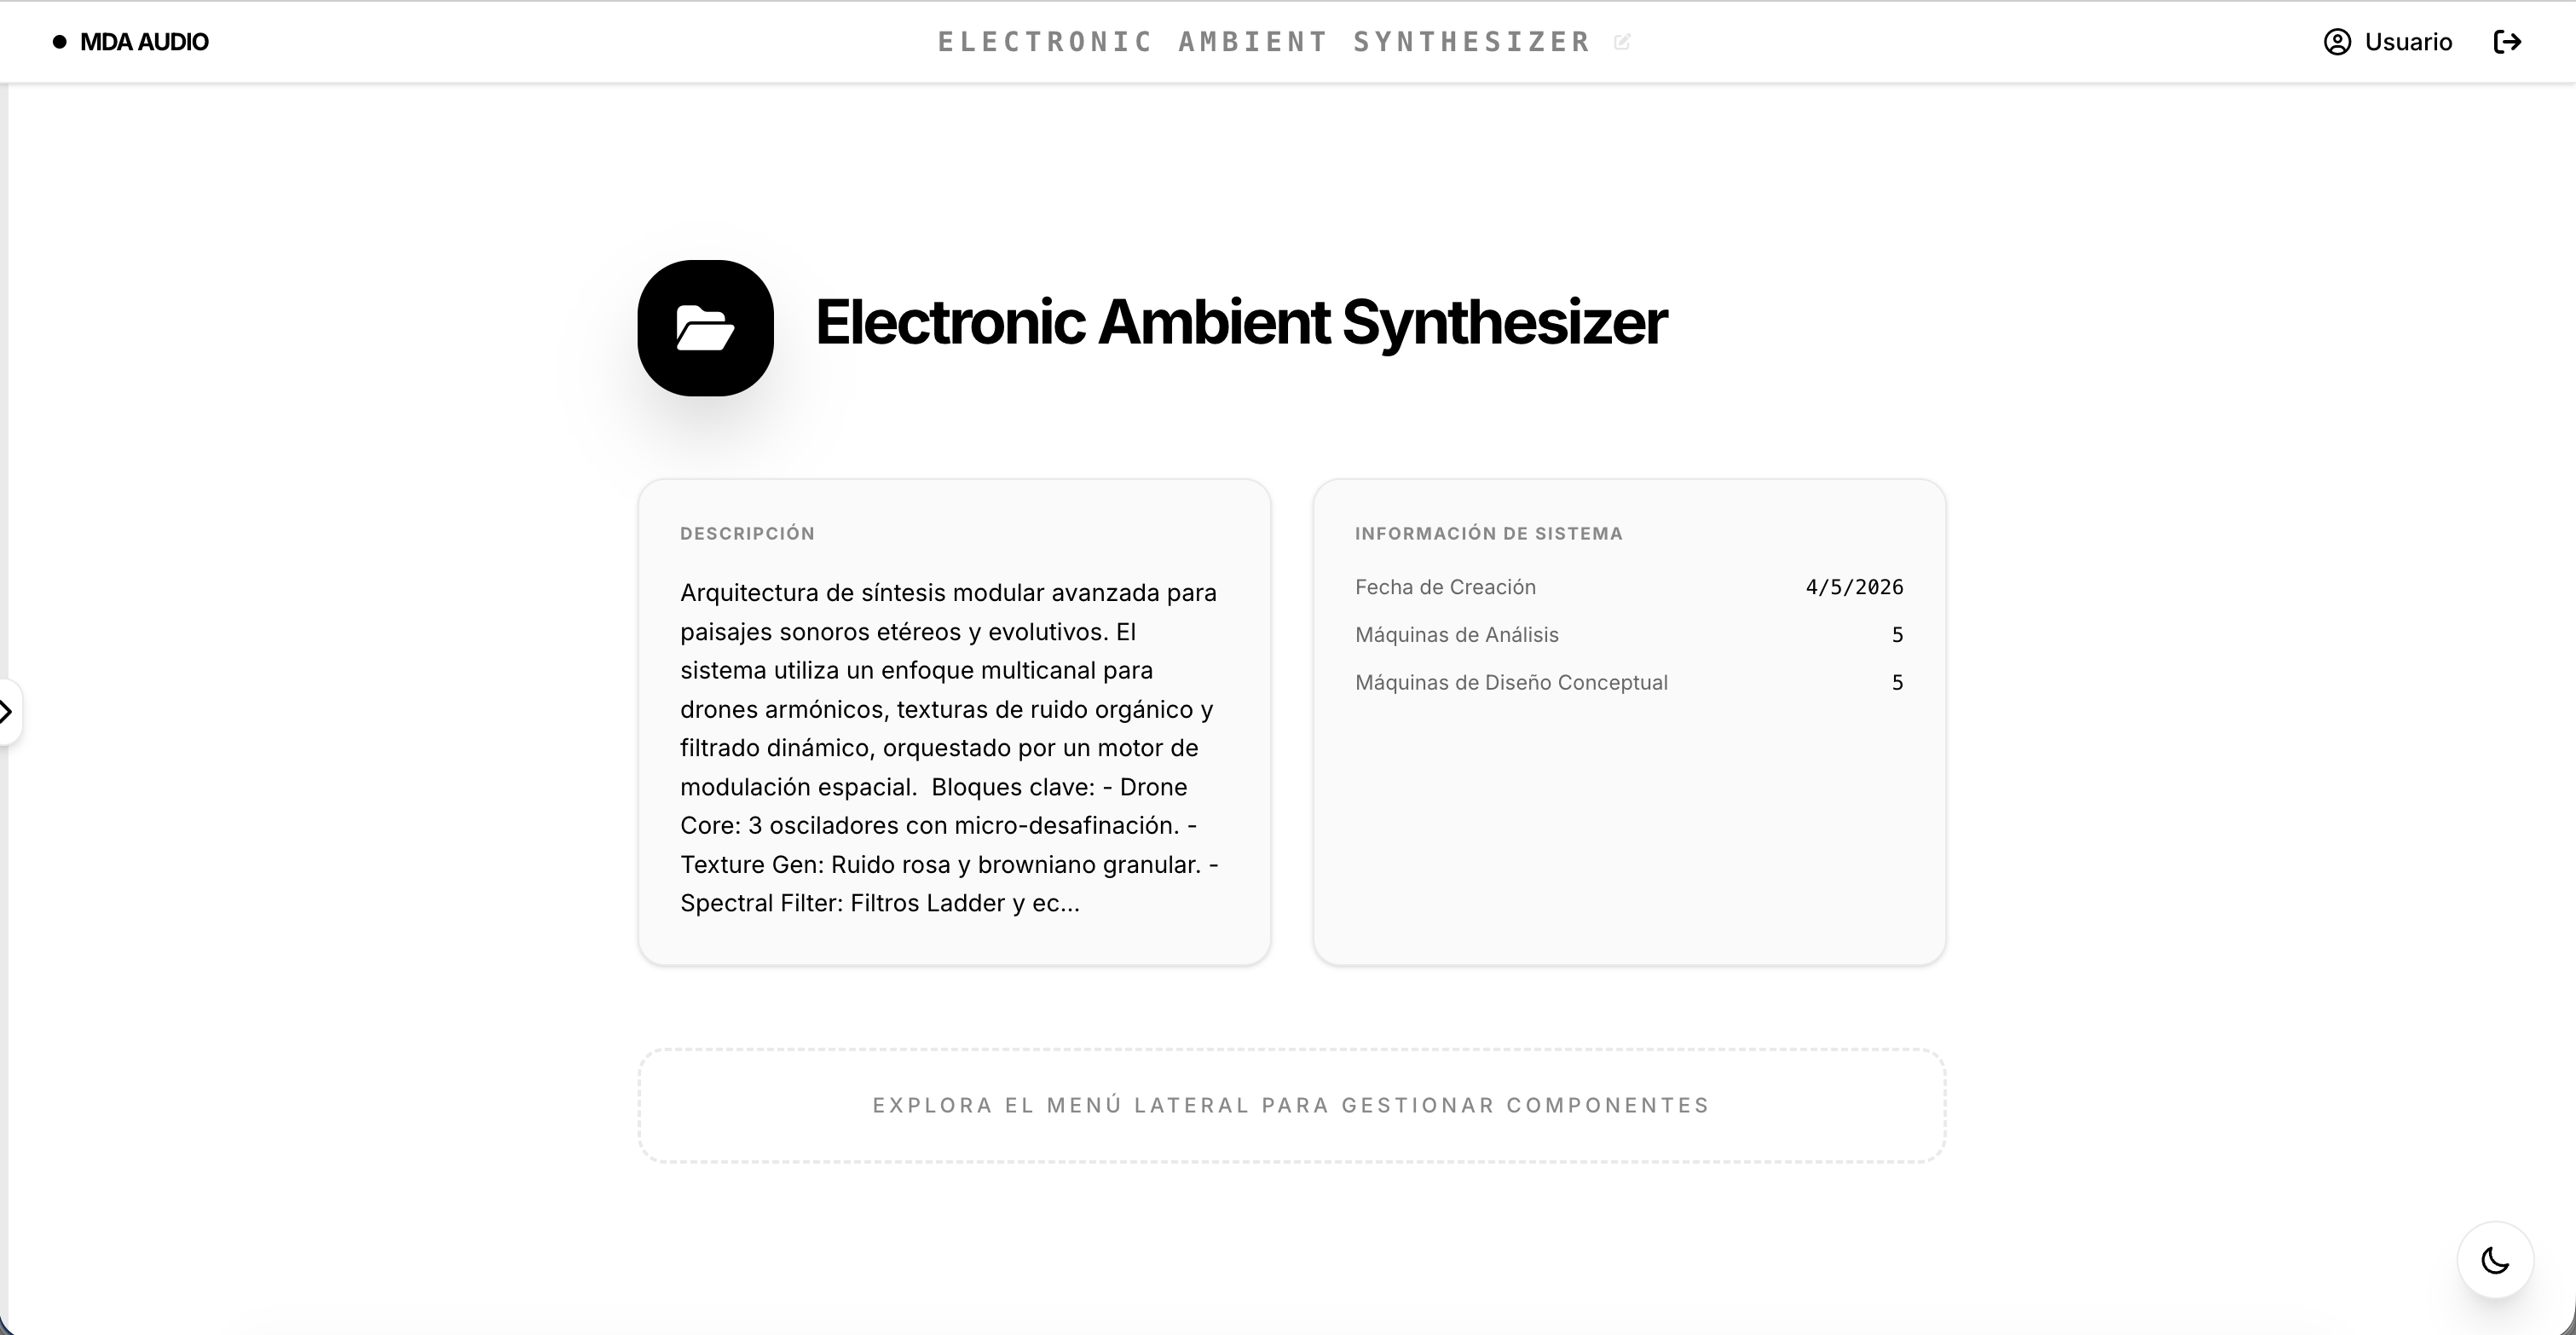
\includegraphics[width=0.6\textwidth]{imagenes/04_estructura/02_ocultacionExplorador.png}
    \caption{Botón para colapsar y ocultar el explorador lateral.}
\end{figure}

Para maximizar el espacio disponible en el área central, especialmente útil durante la edición de esquemas visuales complejos, el explorador puede ser colapsado y ocultado pulsando el botón situado en la parte superior izquierda.

\subsection{Barra Principal y Área de Trabajo}

\begin{figure}[!ht]
    \centering
    
\includegraphics[width=\textwidth]{imagenes/04_estructura/04_barraPrincipal.png}
    \caption{Barra de herramientas principal.}
\end{figure}

La barra principal incluye, además de las opciones de gestión de sesión del usuario, botones de navegación como la vuelta al panel de proyectos y accesos a funcionalidades globales de exportación de modelos.

\begin{figure}[!ht]
    \centering
    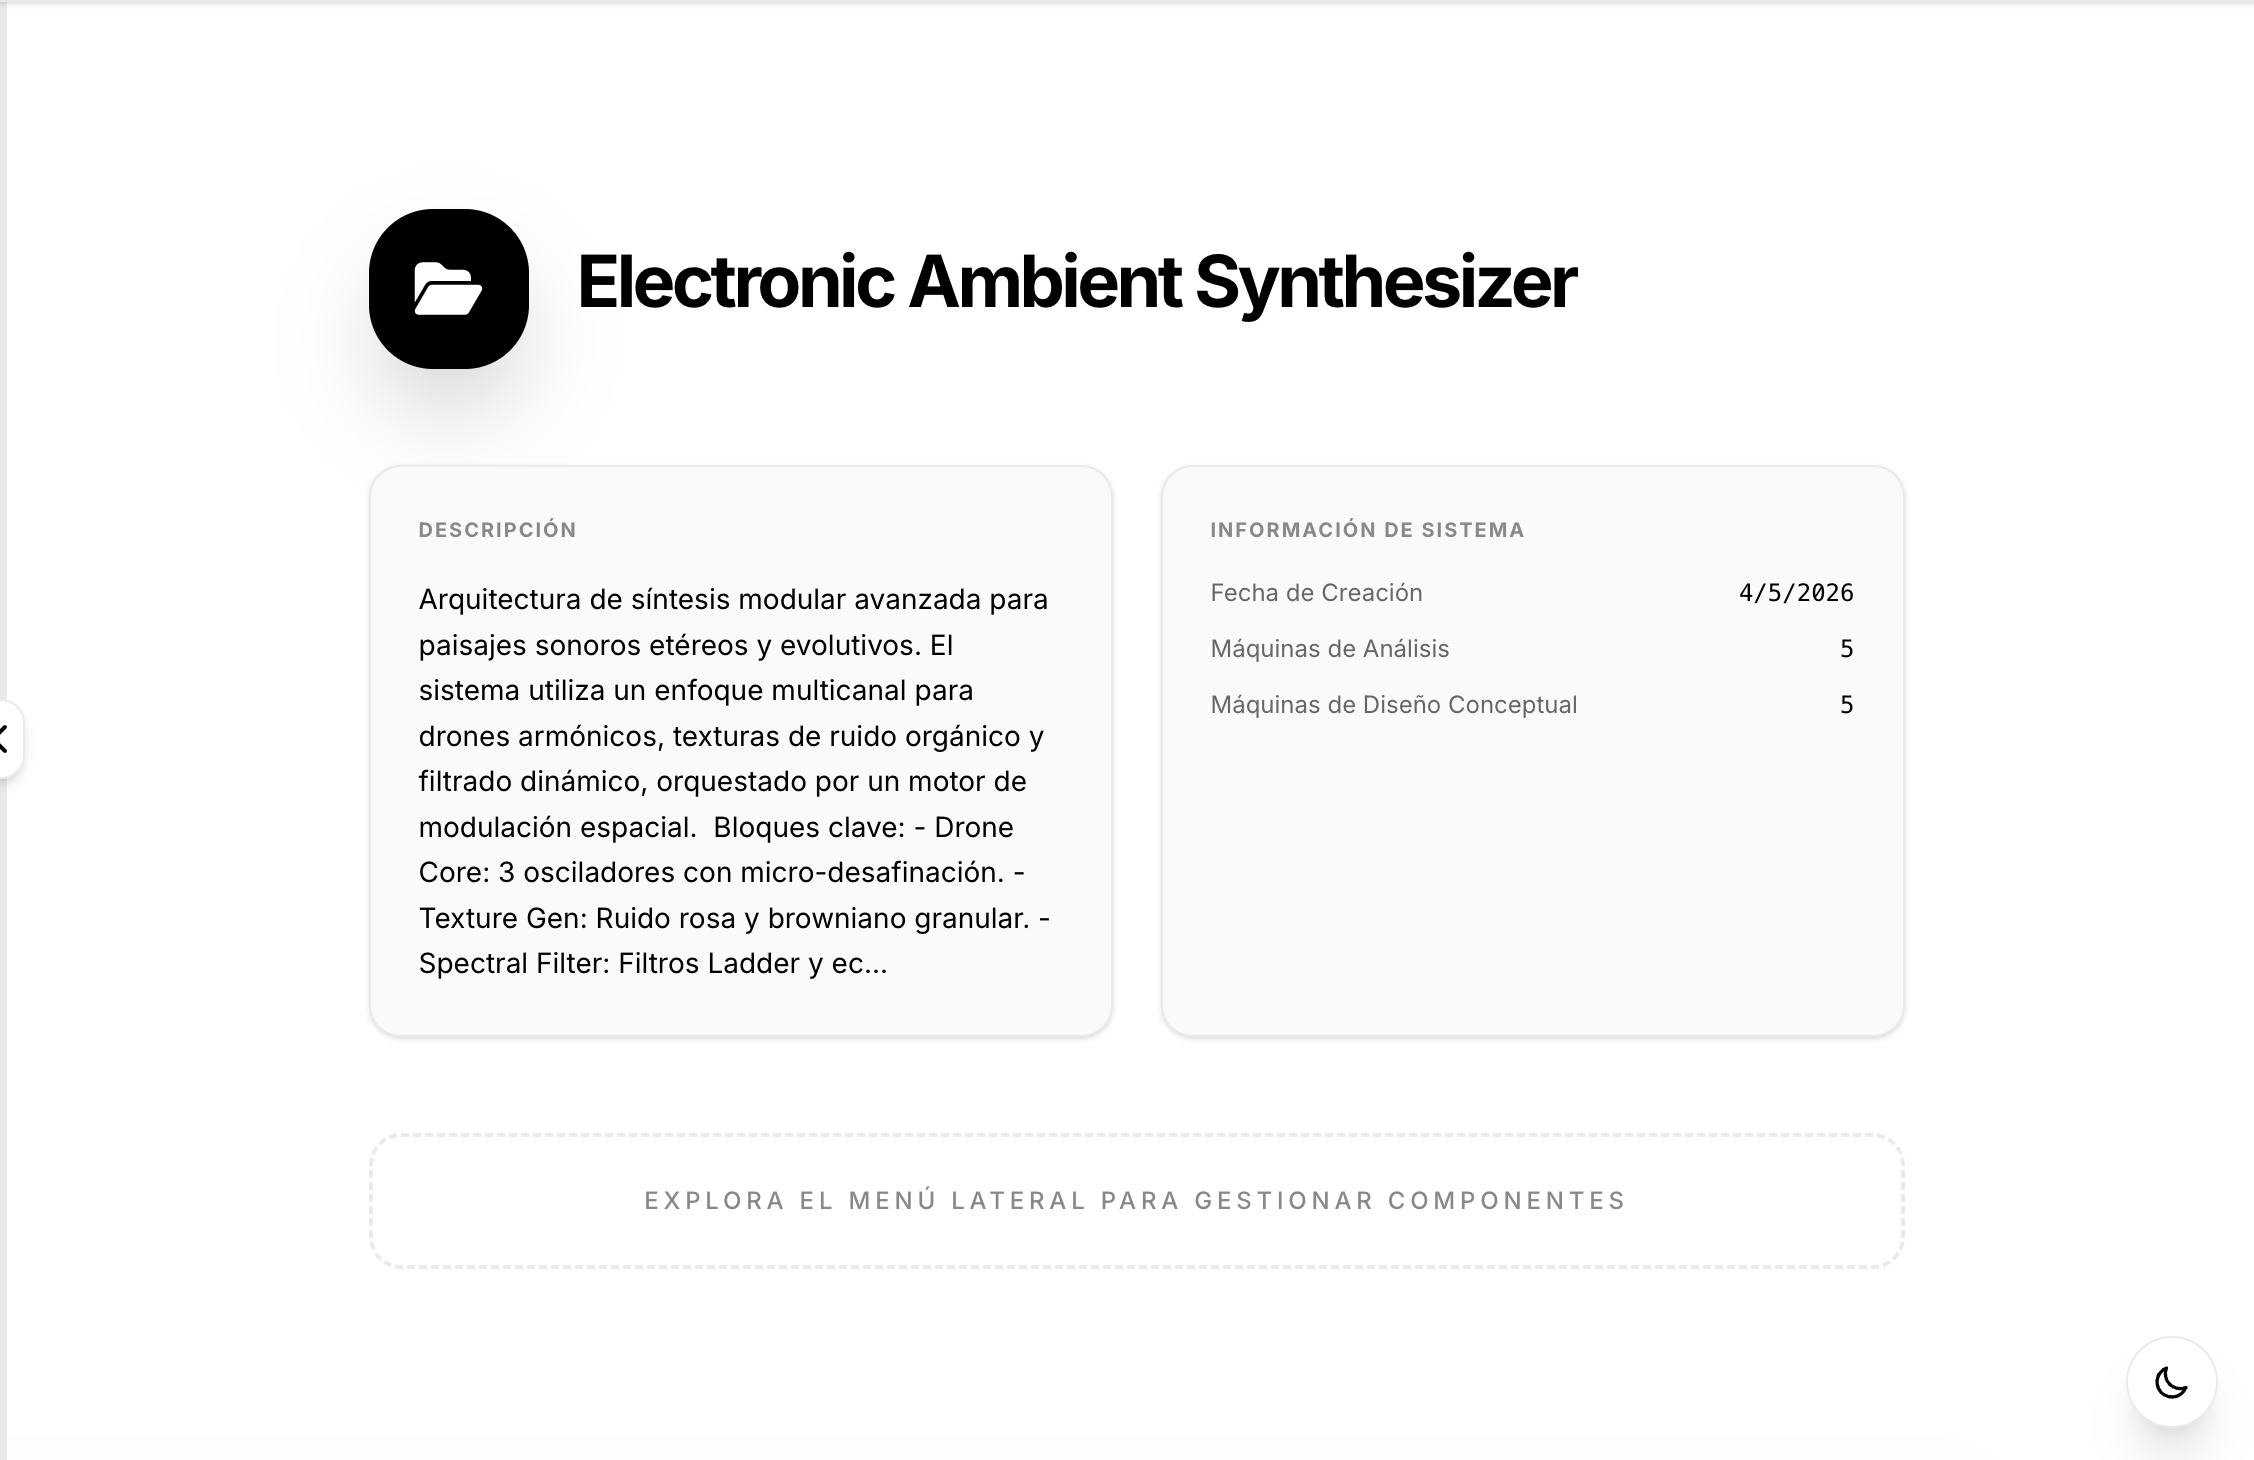
\includegraphics[width=\textwidth]{imagenes/04_estructura/05_objetosAbiertosEnElExplorador.png}
    \caption{Área de trabajo central con múltiples pestañas abiertas.}
\end{figure}

El área central utiliza un sistema de pestañas. A medida que el usuario selecciona elementos en el explorador, estos se abren en nuevas pestañas. Esto permite:
\begin{itemize}
    \item \textbf{Multitarea:} Mantener abiertos simultáneamente modelos de análisis, editores de diseño y grafos de relaciones.
    \item \textbf{Navegación Rápida:} Cambiar de contexto entre un modelo \textit{CIM} y uno \textit{PIM} rápidamente para verificar correspondencias conceptuales.
    \item \textbf{Cierre Selectivo:} Cerrar individualmente las pestañas que ya no se necesiten para mantener ordenado el espacio visual.
\end{itemize}
